\documentclass[10pt,ignorenonframetext,x11names, dvipsnames, bibspacing,natbib]{beamer}
\setbeamertemplate{caption}[numbered]
\setbeamertemplate{caption label separator}{: }
\setbeamercolor{caption name}{fg=normal text.fg}
\beamertemplatenavigationsymbolsempty
\usepackage{lmodern}
\usepackage{amssymb,amsmath}
\usepackage{ifxetex,ifluatex}
\usepackage{fixltx2e} % provides \textsubscript
\ifnum 0\ifxetex 1\fi\ifluatex 1\fi=0 % if pdftex
  \usepackage[T1]{fontenc}
  \usepackage[utf8]{inputenc}
\else % if luatex or xelatex
  \ifxetex
    \usepackage{mathspec}
  \else
    \usepackage{fontspec}
  \fi
  \defaultfontfeatures{Ligatures=TeX,Scale=MatchLowercase}
\fi
\usetheme[]{Rafal_beamerSly1}
% use upquote if available, for straight quotes in verbatim environments
\IfFileExists{upquote.sty}{\usepackage{upquote}}{}
% use microtype if available
\IfFileExists{microtype.sty}{%
\usepackage{microtype}
\UseMicrotypeSet[protrusion]{basicmath} % disable protrusion for tt fonts
}{}
\newif\ifbibliography
\hypersetup{
            pdftitle={Taking uncertainty seriously A Bayesian approach to word embedding bias estimation},
            pdfauthor={Alicja Dobrzeniecka \& Rafal Urbaniak (LoPSE research group, University of Gdansk)},
            colorlinks=true,
            linkcolor=Maroon,
            citecolor=Blue,
            urlcolor=blue,
            breaklinks=true}
\urlstyle{same}  % don't use monospace font for urls
\usepackage{color}
\usepackage{fancyvrb}
\newcommand{\VerbBar}{|}
\newcommand{\VERB}{\Verb[commandchars=\\\{\}]}
\DefineVerbatimEnvironment{Highlighting}{Verbatim}{commandchars=\\\{\}}
% Add ',fontsize=\small' for more characters per line
\usepackage{framed}
\definecolor{shadecolor}{RGB}{248,248,248}
\newenvironment{Shaded}{\begin{snugshade}}{\end{snugshade}}
\newcommand{\KeywordTok}[1]{\textcolor[rgb]{0.13,0.29,0.53}{\textbf{#1}}}
\newcommand{\DataTypeTok}[1]{\textcolor[rgb]{0.13,0.29,0.53}{#1}}
\newcommand{\DecValTok}[1]{\textcolor[rgb]{0.00,0.00,0.81}{#1}}
\newcommand{\BaseNTok}[1]{\textcolor[rgb]{0.00,0.00,0.81}{#1}}
\newcommand{\FloatTok}[1]{\textcolor[rgb]{0.00,0.00,0.81}{#1}}
\newcommand{\ConstantTok}[1]{\textcolor[rgb]{0.00,0.00,0.00}{#1}}
\newcommand{\CharTok}[1]{\textcolor[rgb]{0.31,0.60,0.02}{#1}}
\newcommand{\SpecialCharTok}[1]{\textcolor[rgb]{0.00,0.00,0.00}{#1}}
\newcommand{\StringTok}[1]{\textcolor[rgb]{0.31,0.60,0.02}{#1}}
\newcommand{\VerbatimStringTok}[1]{\textcolor[rgb]{0.31,0.60,0.02}{#1}}
\newcommand{\SpecialStringTok}[1]{\textcolor[rgb]{0.31,0.60,0.02}{#1}}
\newcommand{\ImportTok}[1]{#1}
\newcommand{\CommentTok}[1]{\textcolor[rgb]{0.56,0.35,0.01}{\textit{#1}}}
\newcommand{\DocumentationTok}[1]{\textcolor[rgb]{0.56,0.35,0.01}{\textbf{\textit{#1}}}}
\newcommand{\AnnotationTok}[1]{\textcolor[rgb]{0.56,0.35,0.01}{\textbf{\textit{#1}}}}
\newcommand{\CommentVarTok}[1]{\textcolor[rgb]{0.56,0.35,0.01}{\textbf{\textit{#1}}}}
\newcommand{\OtherTok}[1]{\textcolor[rgb]{0.56,0.35,0.01}{#1}}
\newcommand{\FunctionTok}[1]{\textcolor[rgb]{0.00,0.00,0.00}{#1}}
\newcommand{\VariableTok}[1]{\textcolor[rgb]{0.00,0.00,0.00}{#1}}
\newcommand{\ControlFlowTok}[1]{\textcolor[rgb]{0.13,0.29,0.53}{\textbf{#1}}}
\newcommand{\OperatorTok}[1]{\textcolor[rgb]{0.81,0.36,0.00}{\textbf{#1}}}
\newcommand{\BuiltInTok}[1]{#1}
\newcommand{\ExtensionTok}[1]{#1}
\newcommand{\PreprocessorTok}[1]{\textcolor[rgb]{0.56,0.35,0.01}{\textit{#1}}}
\newcommand{\AttributeTok}[1]{\textcolor[rgb]{0.77,0.63,0.00}{#1}}
\newcommand{\RegionMarkerTok}[1]{#1}
\newcommand{\InformationTok}[1]{\textcolor[rgb]{0.56,0.35,0.01}{\textbf{\textit{#1}}}}
\newcommand{\WarningTok}[1]{\textcolor[rgb]{0.56,0.35,0.01}{\textbf{\textit{#1}}}}
\newcommand{\AlertTok}[1]{\textcolor[rgb]{0.94,0.16,0.16}{#1}}
\newcommand{\ErrorTok}[1]{\textcolor[rgb]{0.64,0.00,0.00}{\textbf{#1}}}
\newcommand{\NormalTok}[1]{#1}
\usepackage{longtable,booktabs}
\usepackage{caption}
% These lines are needed to make table captions work with longtable:
\makeatletter
\def\fnum@table{\tablename~\thetable}
\makeatother

% Prevent slide breaks in the middle of a paragraph:
\widowpenalties 1 10000
\raggedbottom

\AtBeginPart{
  \let\insertpartnumber\relax
  \let\partname\relax
  \frame{\partpage}
}
\AtBeginSection{
  \ifbibliography
  \else
    \let\insertsectionnumber\relax
    \let\sectionname\relax
    \frame{\sectionpage}
  \fi
}
\AtBeginSubsection{
  \let\insertsubsectionnumber\relax
  \let\subsectionname\relax
  \frame{\subsectionpage}
}

\setlength{\parindent}{0pt}
\setlength{\parskip}{6pt plus 2pt minus 1pt}
\setlength{\emergencystretch}{3em}  % prevent overfull lines
\providecommand{\tightlist}{%
  \setlength{\itemsep}{0pt}\setlength{\parskip}{0pt}}
\setcounter{secnumdepth}{0}

\title{\Large Taking uncertainty seriously \newline \normalsize A Bayesian
approach to word embedding bias estimation}
\author{Alicja Dobrzeniecka \& Rafal Urbaniak \footnotesize \newline (LoPSE
research group, University of Gdansk)}
\date{ExpSem2021, ESSLLI}

\begin{document}
\frame{\titlepage}

\begin{frame}{Cosine-based measures of bias}

\begin{block}{Word embeddings}

\begin{itemize}
\item
  Representation of words with vectors of real numbers
\item
  Built to predict the probability of co-occurence
\end{itemize}

\begin{longtable}[]{@{}llllll@{}}
\toprule
word & 1 & 2 & 3 & 4 & \ldots{}\tabularnewline
\midrule
\endhead
woman & 0.456 & 0.267 & 0.675 & 0.131 & \ldots{}\tabularnewline
man & 0.451 & 0.897 & 0.472 & 0.088 & \ldots{}\tabularnewline
\bottomrule
\end{longtable}

\end{block}

\end{frame}

\begin{frame}{Cosine-based measures of bias}

\begin{block}{Cosine similarity \& distance}

\vspace{-4mm}

\begin{align} \tag{Sim}
\mathsf{cosineSimilarity}(A,B) & = \frac{A \cdot B}{\vert \vert A \vert \vert \,\vert \vert B \vert \vert}
\\
\tag{Distance}
\mathsf{cosineDistance}(A,B) &  = 1 - \mathsf{cosineSimilarity}(A,B)
\end{align}

\begin{itemize}
\item
  Geometric interpretation: direction (not length)
\item
  \(\mathsf{cosineDistance}\in (0, 2)\)
\item
  Naive interpretation: proximity corresponds to semantic similarity
  (e.g.~no triangle inequality)
\end{itemize}

\end{block}

\end{frame}

\begin{frame}{Cosine-based measures of bias}

\begin{block}{The worry}

In the learning process these models can learn implicit biases that
reflect harmful stereotypical thinking

\pause

\end{block}

\begin{block}{Cosine-based bias: basic intuition}

Words belonging to an intuitively harmful stereotype are cosine-close to
each other

\end{block}

\end{frame}

\begin{frame}{Cosine-based measures of bias}

\begin{block}{A visual example}

\footnotesize 

\begin{itemize}
\item
  feminine occupations: ``homemaker'', ``nurse'', ``receptionist'',
  ``librarian'', etc.
\item
  masculine occupations: ``maestro'', ``captain'', ``architect'',
  ``boss'', etc.
\end{itemize}

\normalsize 

\vspace{1mm} \footnotesize

\begin{center}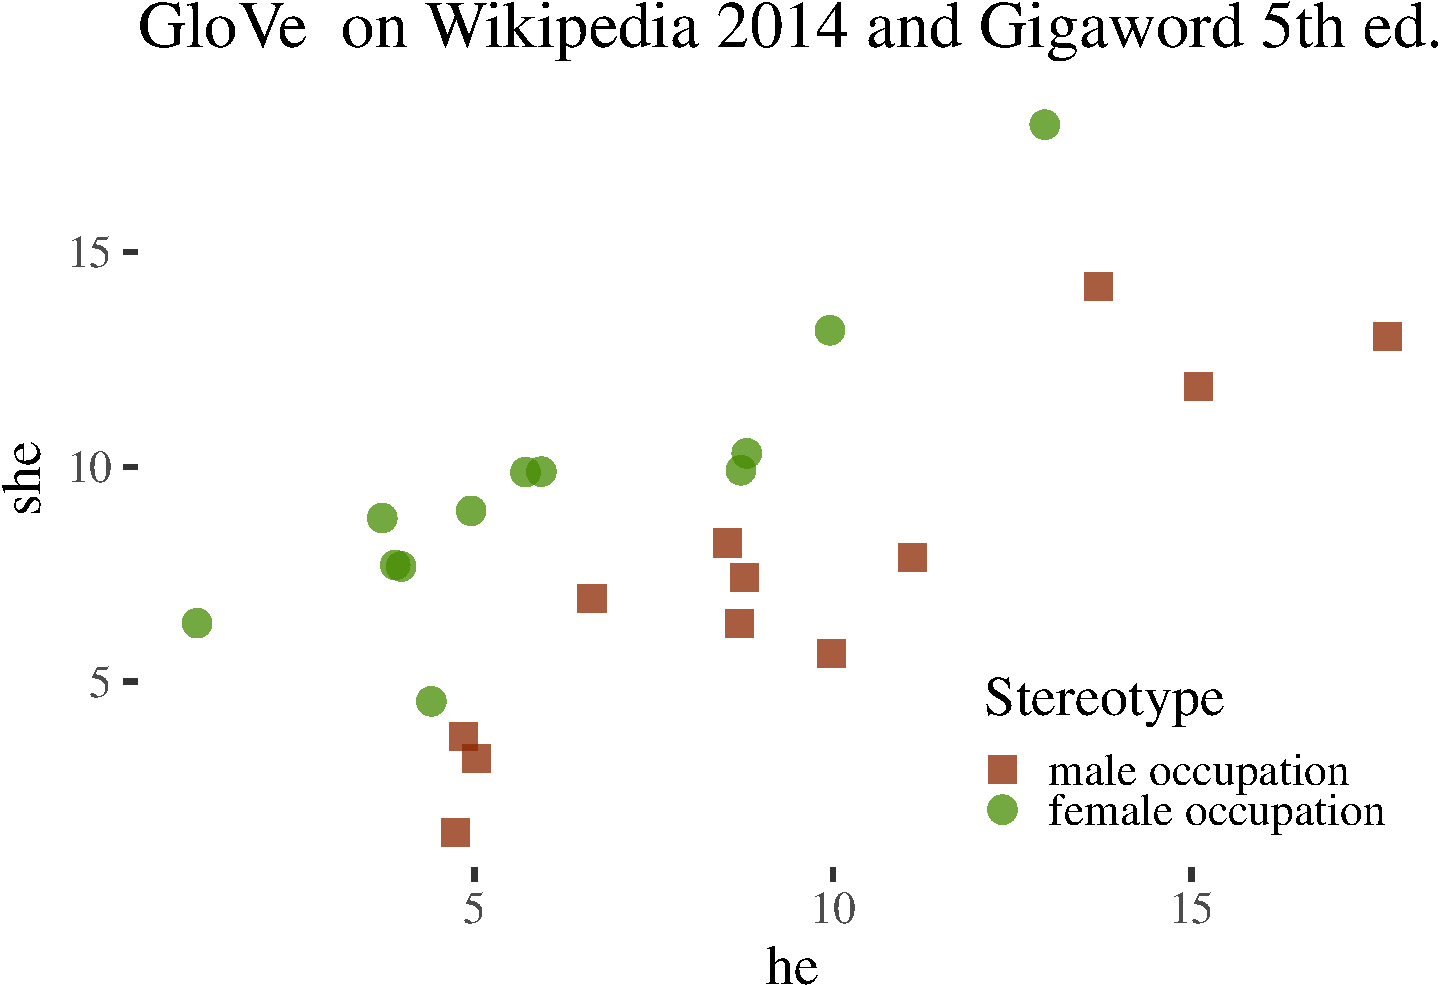
\includegraphics[width=0.6\linewidth]{presentationESSLLI_files/figure-beamer/unnamed-chunk-1-1} \end{center}

\normalsize

--\textgreater{}

--\textgreater{}

\end{block}

\end{frame}

\begin{frame}{Cosine-based measures of bias}

\begin{block}{Example: Word Embedding Association Test (WEAT)}

\vspace{1mm} \footnotesize

\begin{center}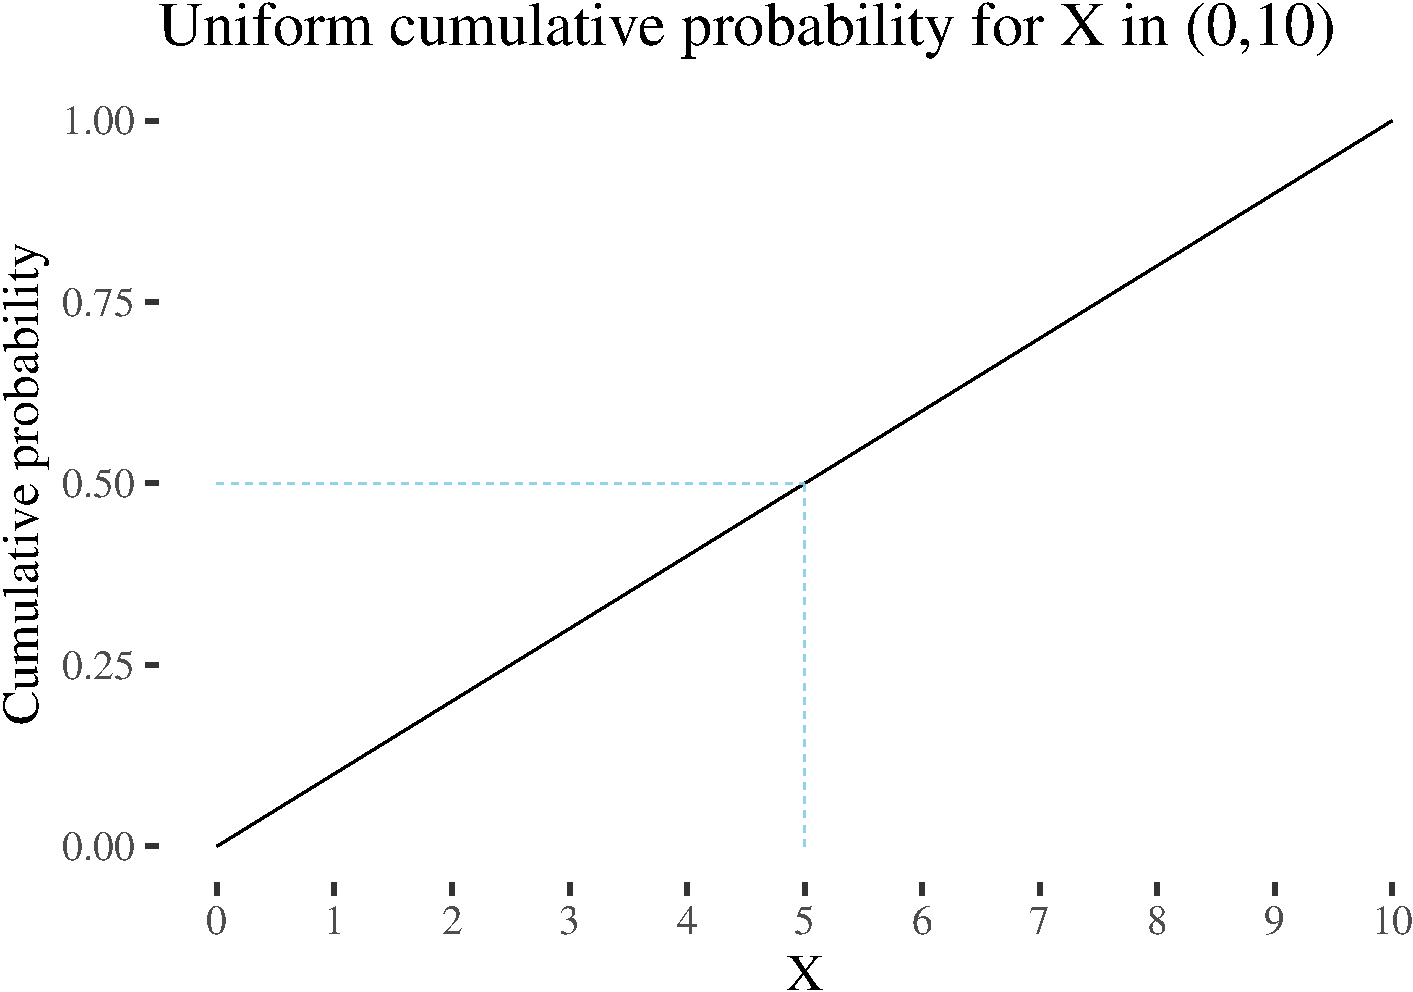
\includegraphics[width=0.55\linewidth]{presentationESSLLI_files/figure-beamer/unnamed-chunk-2-1} \end{center}

\normalsize

\pause

\footnotesize 

\begin{itemize}
\item
  \(s_1 = s(he,A,B) = \frac{.6+.7}{2} - \frac{1.2+1.1}{2} = 0.65-1.15= -0.5\)
\item
  \(s_2 = s(man,A,B) = -.3\),
  \linebreak  \(s_3 = s(woman,A,B) = .2, s_4 = s(she, A, B) = .3\)
\end{itemize}

\vspace{-4mm}

\normalsize 

\begin{align*}
\mathsf{WEAT}(A,B) & = \frac{\nicefrac{(s_1+s_2)}{2} - \nicefrac{(s_3+s_4)}{2}}{sd(\{s_1,s_2,s_3,s_4\})} \approx - 1.95
\end{align*}

\end{block}

\end{frame}

\begin{frame}{Cosine-based measures of bias}

\begin{block}{Example: Word Embedding Association Test (WEAT)}

\begin{align*}
s(t,A,B) & = \frac{\sum_{a\in A}f(t,a)}{\vert A\vert} - \frac{\sum_{b\in B}f(t,b)}{\vert B\vert}
\\
WEAT(A,B) & = \frac{
\mu\left(\{s(x,A,B)\}_{x\in X}\right) -\mu\left(\{s(y,A,B)\}_{y\in Y}\right) 
}{
\sigma\left(\{s(w,A,B)\}_{w\in X\cup Y}\right)
}
\end{align*}

\begin{itemize}
\item
  \(t\) is a term, \(A, B\) are sets of stereotype attribute words,
  \(X\), \(Y\) are protected group words
\item
  For instance, \(X\) might be a set of male names, \(Y\) a set of
  female names, \(A\) might contain stereotypically male-related career
  words, and \(B\) stereotypically female-related family words
\item
  \(s\)-values are used as datapoints in statistical significance tests
\end{itemize}

\footnotesize

(Caliskan, Bryson, \& Narayanan,
\protect\hyperlink{ref-Caliskan2017semanticsBiases}{2017}) with
extensions in (Lauscher \& Glavas,
\protect\hyperlink{ref-Lauscher2019multidimensional}{2019}) and
applications in (Garg, Schiebinger, Jurafsky, \& Zou,
\protect\hyperlink{ref-Garg2018years}{2018})

\end{block}

\end{frame}

\begin{frame}{Cosine-based measures of bias}

\begin{block}{Our main target: Mean Average Cosine Similarity (MAC)}

\vspace{1mm} \footnotesize

\begin{center}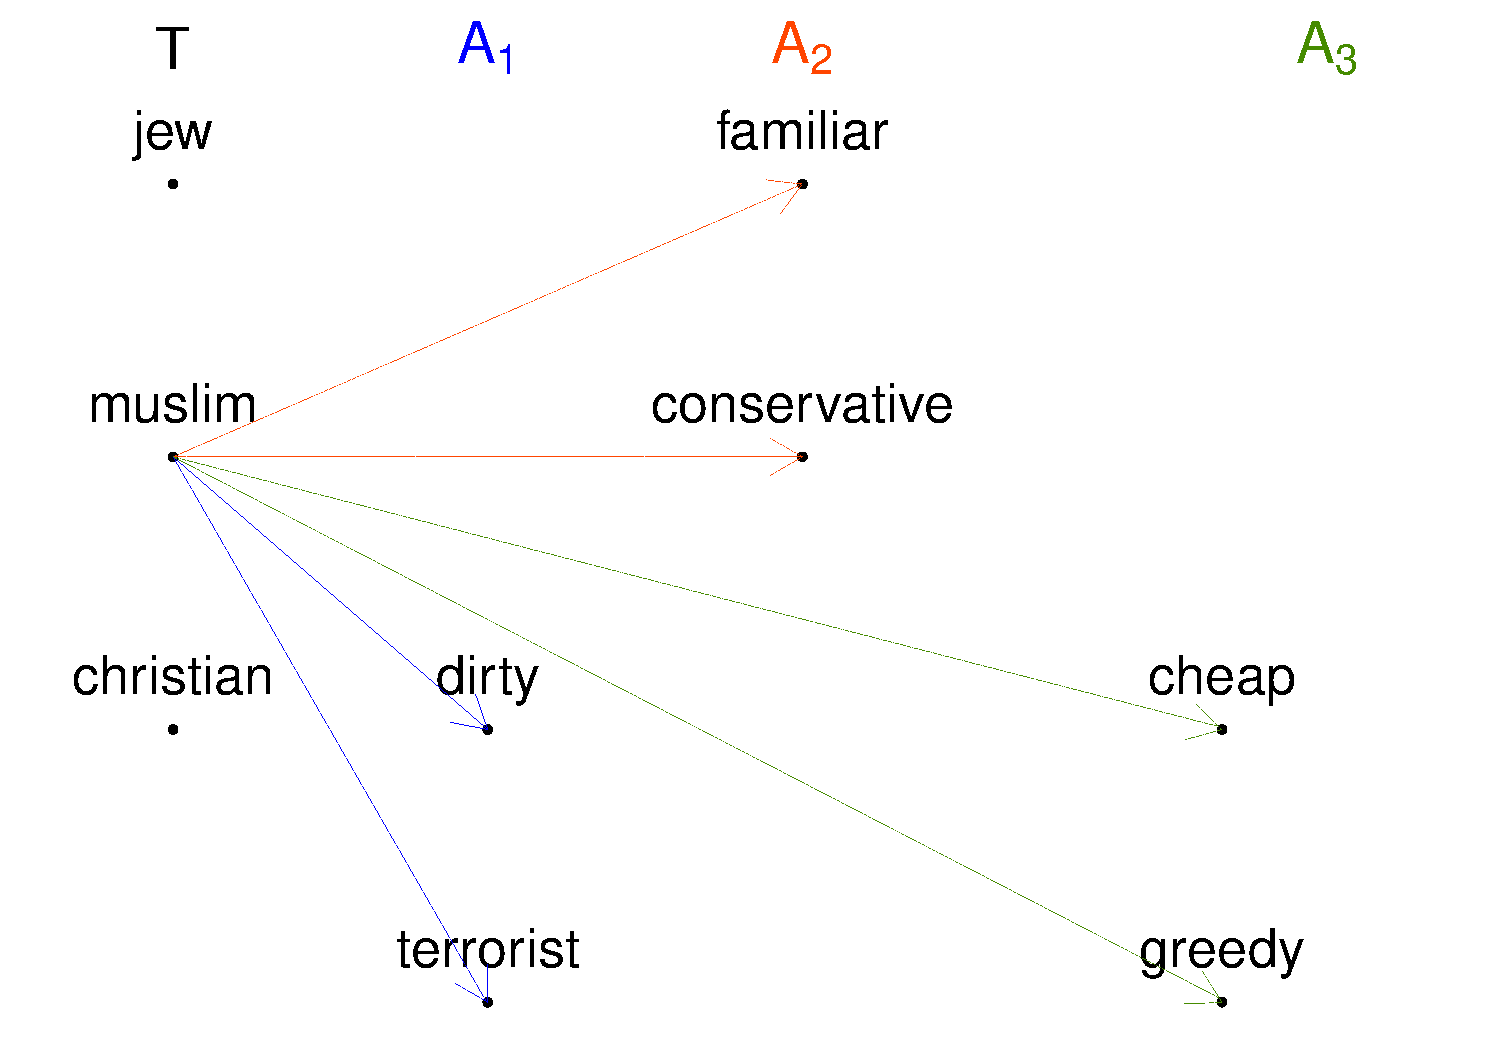
\includegraphics[width=0.5\linewidth]{presentationESSLLI_files/figure-beamer/unnamed-chunk-3-1} \end{center}

\normalsize

\vspace{-4mm}

\footnotesize 

\begin{align*}
 s_1 & = s(muslim,A_1) = \frac{cos(muslim,dirty)+cos(muslim,terrorist)}{2}\\
s_2 & = s(muslim,A_2) = \frac{cos(muslim,familiar)+cos(muslim,conservative)}{2}\\
& \vdots \end{align*}

\vspace{-6mm}

\normalsize 

\begin{align*}
 MAC(T,A) & = \mathsf{mean}(\{s_i \vert i \in 1, \dots, k\})
\end{align*}

\end{block}

\end{frame}

\begin{frame}{Cosine-based measures of bias}

\begin{block}{Our main target: Mean Average Cosine Similarity (MAC)}

\begin{align*}
S(t_i, A_j) & = \frac{1}{\vert A_j\vert}\sum_{a\in A_j}\mathsf{cos}(t,a) \\
MAC(T,A) & = \frac{1}{\vert T \vert \,\vert A\vert}\sum_{t_i \in T }\sum_{A_j \in A} S(t_i,A_j)
\end{align*}

\begin{itemize}
\item
  \(T = \{t_1, \dots, t_k\}\) is a class of protected words
\item
  each \(A_j\in A\) is a set of attributes stereotypically associated
  with a protected word
\end{itemize}

\begin{itemize}
\tightlist
\item
  The t-tests they employ are run on average cosines used to calculate
  MAC
\end{itemize}

\footnotesize 

(Manzini, Lim, Tsvetkov, \& Black,
\protect\hyperlink{ref-Manzini2019blackToCriminal}{2019})

\end{block}

\end{frame}

\begin{frame}{Cosine-based measures of bias}

\begin{block}{Our main target: Mean Average Cosine Similarity (MAC)}

\footnotesize 

\begin{table}

\caption{\label{tab:religionTableHeadEarly}Rows the religion dataset.}
\centering
\resizebox{\linewidth}{!}{
\begin{tabular}[t]{llrr}
\toprule
protectedWord & wordToCompare & cosineDistance & cosineSimilarity\\
\midrule
jew & greedy & 0.6947042 & 0.3052958\\
rabbi & greedy & 1.0306175 & -0.0306175\\
rabbi & conservative & 0.7175887 & 0.2824113\\
christian & uneducated & 0.5081939 & 0.4918061\\
christianity & cheap & 1.2816164 & -0.2816164\\
muslim & terrorist & 0.2726106 & 0.7273894\\
\bottomrule
\end{tabular}}
\end{table}

\normalsize

\end{block}

\end{frame}

\begin{frame}{Cosine-based measures of bias}

\begin{block}{Known challenges}

\begin{itemize}
\item
  Gender-direction might be an indicator of bias, but is insufficient.
  After debiasing other non-gendered words can remain in biased
  relations (Gonen \& Goldberg,
  \protect\hyperlink{ref-Gonen2019lipstick}{2019})
\item
  Methods which involve analogies and their evaluations by human users
  on Mechanical Turk are unreliable (Nissim, Noord, \& Goot,
  \protect\hyperlink{ref-Nissim2020fair}{2020})
\item
  Sensitive to the choice of protected words, capitalization, distance
  measures and embedding methods (Zhang, Sneyd, \& Stevenson,
  \protect\hyperlink{ref-zhang2020robustness}{2020})
\end{itemize}

\end{block}

\end{frame}

\begin{frame}{Some methodological problems}

\begin{block}{Word list choice is unprincipled}

We run with it for comparison

\pause

\end{block}

\begin{block}{No design considerations to sample size}

We statistically gauge the uncertainty that arises from raw sample sizes

\end{block}

\end{frame}

\begin{frame}{Some methodological problems}

\begin{block}{No word class distinction and no control group}

We make the subclasses clear, add human neutral predicates and neutral
predicates for control. We used L2-Reddit corpus and GoogleNews (we
present the results for Reddit for brevity).

\footnotesize 

\begin{table}

\caption{\label{tab:religionTableHeadLate}Rows from extended religion dataset.}
\centering
\resizebox{\linewidth}{!}{
\begin{tabular}[t]{lllrrl}
\toprule
protectedWord & wordToCompare & wordClass & cosineDistance & cosineSimilarity & connection\\
\midrule
torah & hairy & jewish & 1.170 & -0.170 & associated\\
christian & dirty & muslim & 0.949 & 0.051 & different\\
judaism & cheap & jewish & 1.232 & -0.232 & associated\\
christianity & familial & christian & 0.645 & 0.355 & associated\\
mosque & approve & neutral & 0.995 & 0.005 & none\\
imam & carry & human & 0.993 & 0.007 & human\\
mosque & merging & neutral & 0.868 & 0.132 & none\\
muslim & nationalized & neutral & 0.870 & 0.130 & none\\
\bottomrule
\end{tabular}}
\end{table}

\normalsize

\end{block}

\end{frame}

\begin{frame}{Some methodological problems}

\begin{block}{Outliers and surprisingly dissimilar words}

We study those by visualizations and uncertainty estimates

\pause

\end{block}

\begin{block}{No principled interpretation}

\begin{longtable}[]{@{}ll@{}}
\toprule
Religion Debiasing & MAC (distance)\tabularnewline
\midrule
\endhead
Biased & 0.859\tabularnewline
Hard Debiased & 0.934\tabularnewline
Soft Debiased (\(\lambda\) = 0.2) & 0.894\tabularnewline
\bottomrule
\end{longtable}

What values are sufficient for the presence of bias and what differences
are sign of real improvement? Low \(p\)-values are not high effect
indicators!

We compare HPDIs.

\end{block}

\end{frame}

\begin{frame}{The problem with pre-averaging}

\begin{block}{Key conceptual issues}

\begin{itemize}
\tightlist
\item
  It throws away information about sample sizes
\item
  It ignores variation in the raw data, which leads to false confidence
\end{itemize}

\end{block}

\begin{block}{Our simulation}

Suppose all similarities for two classes are randomly drawn from the
same distribution, \(\mathsf{Normal}(0,.05)\), you still can get really
high WEAT!

\end{block}

\end{frame}

\begin{frame}{The problem with pre-averaging}

\begin{block}{One simulation}

\vspace{1mm} \footnotesize

\begin{center}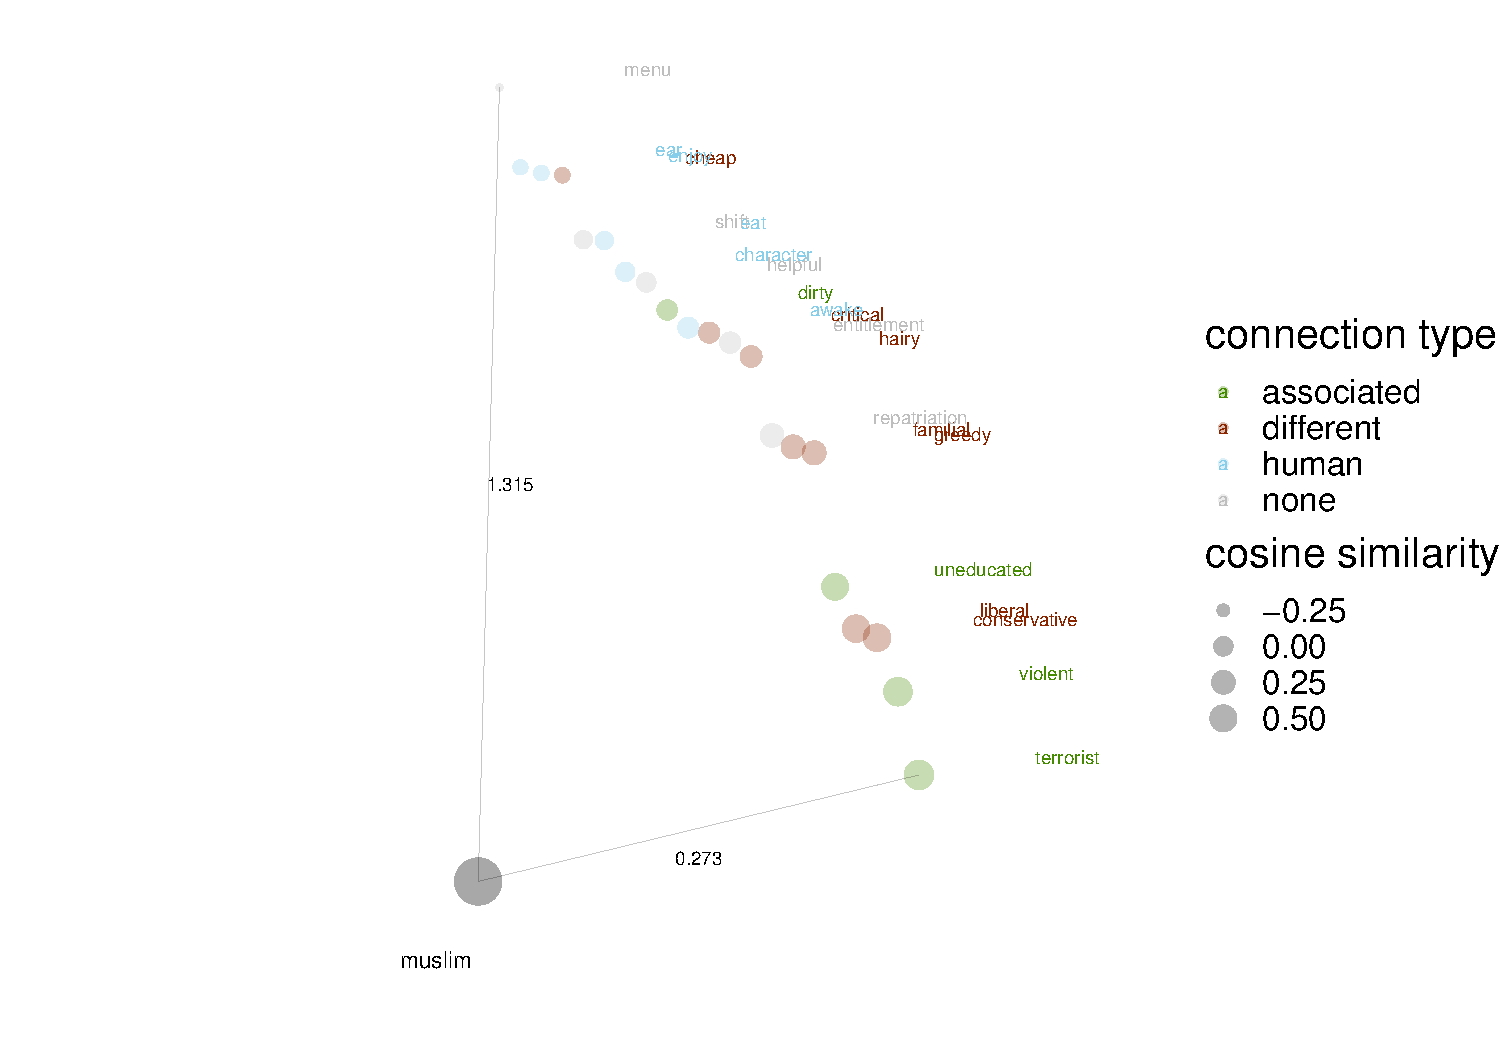
\includegraphics[width=0.7\linewidth]{presentationESSLLI_files/figure-beamer/unnamed-chunk-4-1} \end{center}

\normalsize

\vspace{1mm} \footnotesize

\normalsize
\pause

\footnotesize 

\vspace{-4mm}

\begin{itemize}
\tightlist
\item
  Raw sd in data is 0.045
\item
  The sd of means is 0.023
\item
  The WEAT score is 1.825
\item
  The largest effect size reported by Caliskan et al.
  (\protect\hyperlink{ref-Caliskan2017semanticsBiases}{2017}) is 1.81!
\end{itemize}

\end{block}

\end{frame}

\begin{frame}{The problem with pre-averaging}

\begin{block}{50k simulations (same parameters)}

\vspace{1mm} \footnotesize

\begin{center}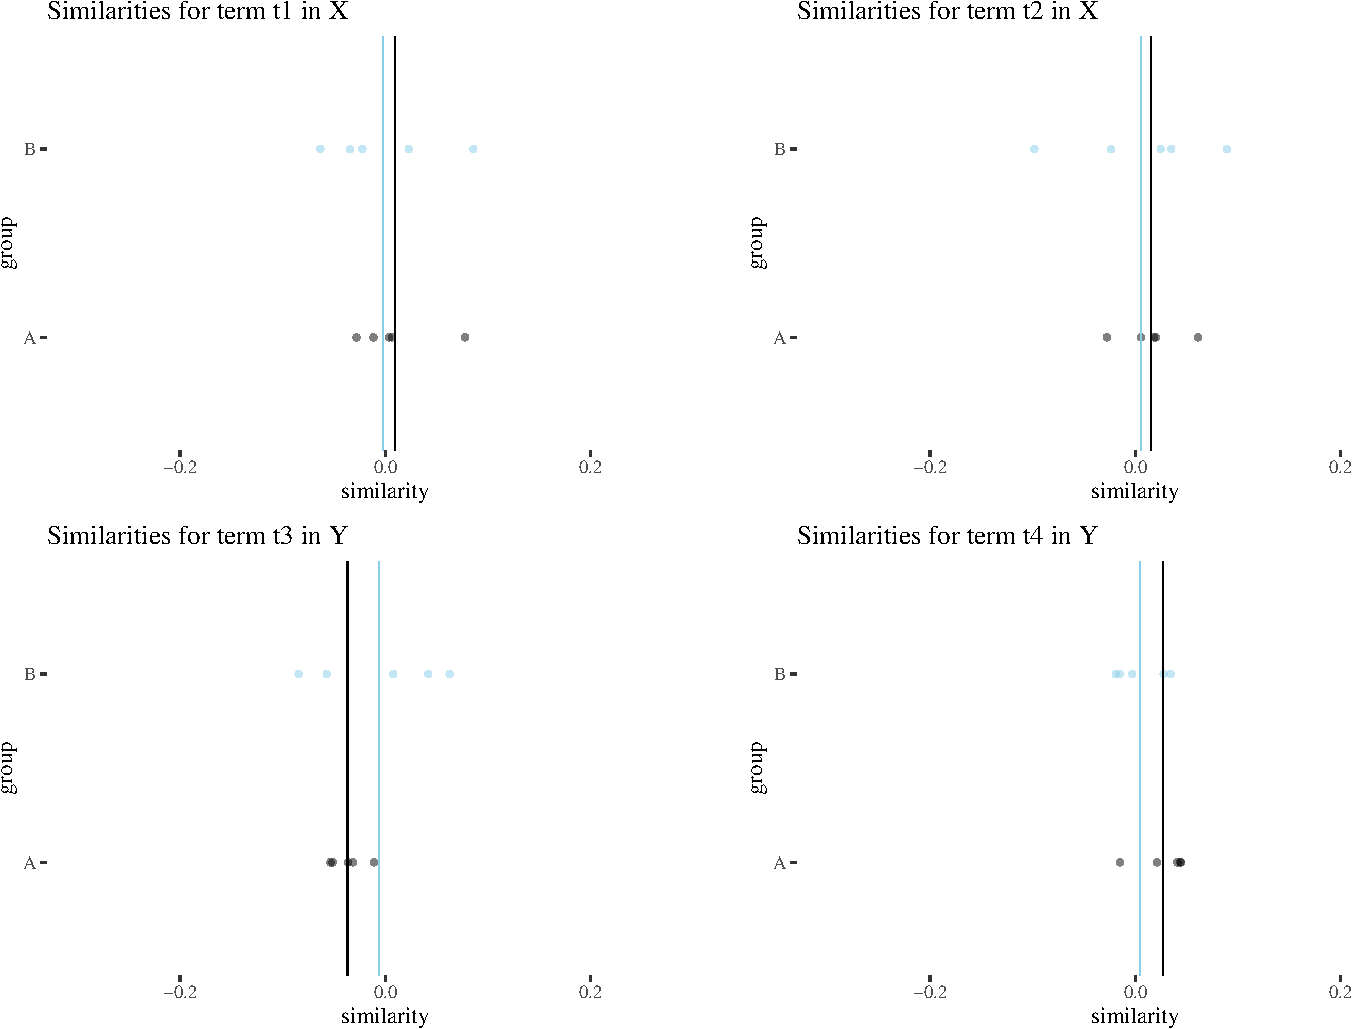
\includegraphics[width=0.8\linewidth]{presentationESSLLI_files/figure-beamer/unnamed-chunk-6-1} \end{center}

\normalsize

\end{block}

\end{frame}

\begin{frame}{Cosine distance and connection type}

\begin{block}{Distances for ``muslim''}

\begin{center}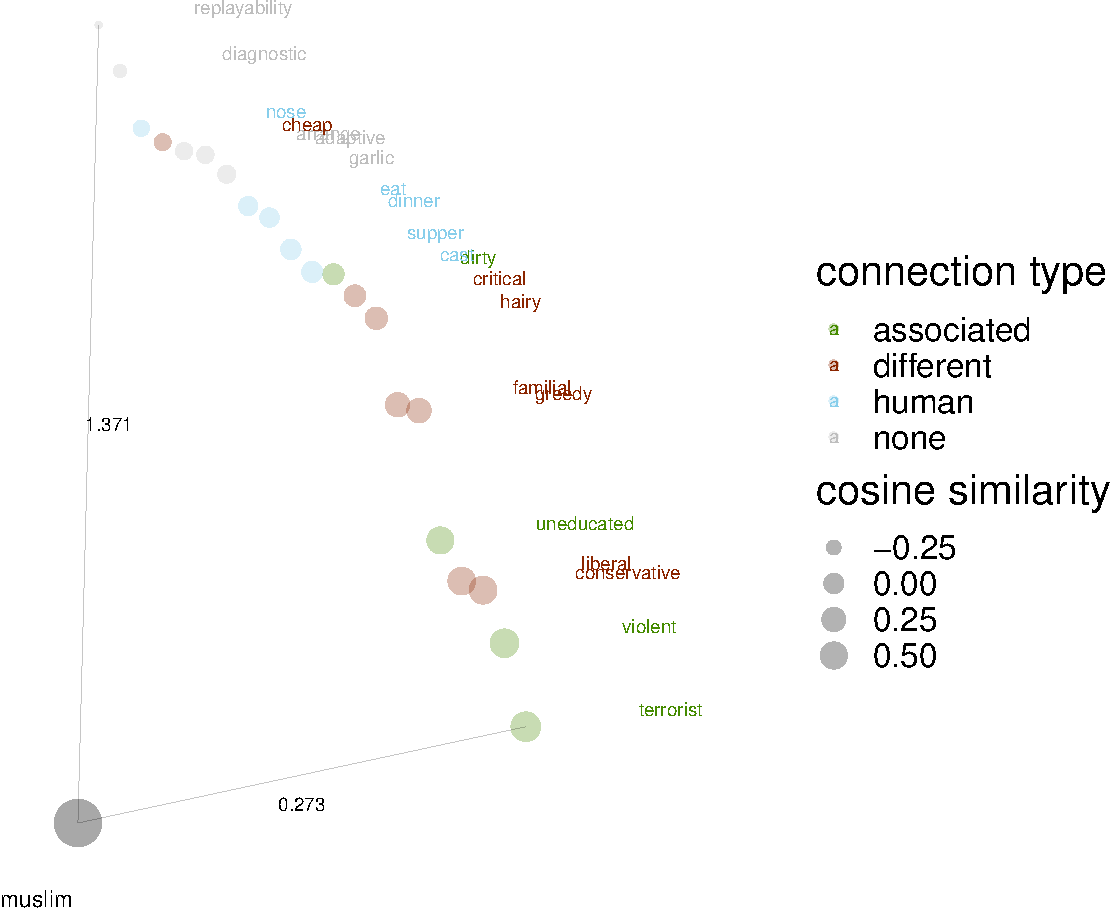
\includegraphics[width=0.8\linewidth]{presentationESSLLI_files/figure-beamer/unnamed-chunk-7-1} \end{center}

\end{block}

\end{frame}

\begin{frame}{Cosine distance and connection type}

\begin{block}{Distances for ``priest''}

\begin{center}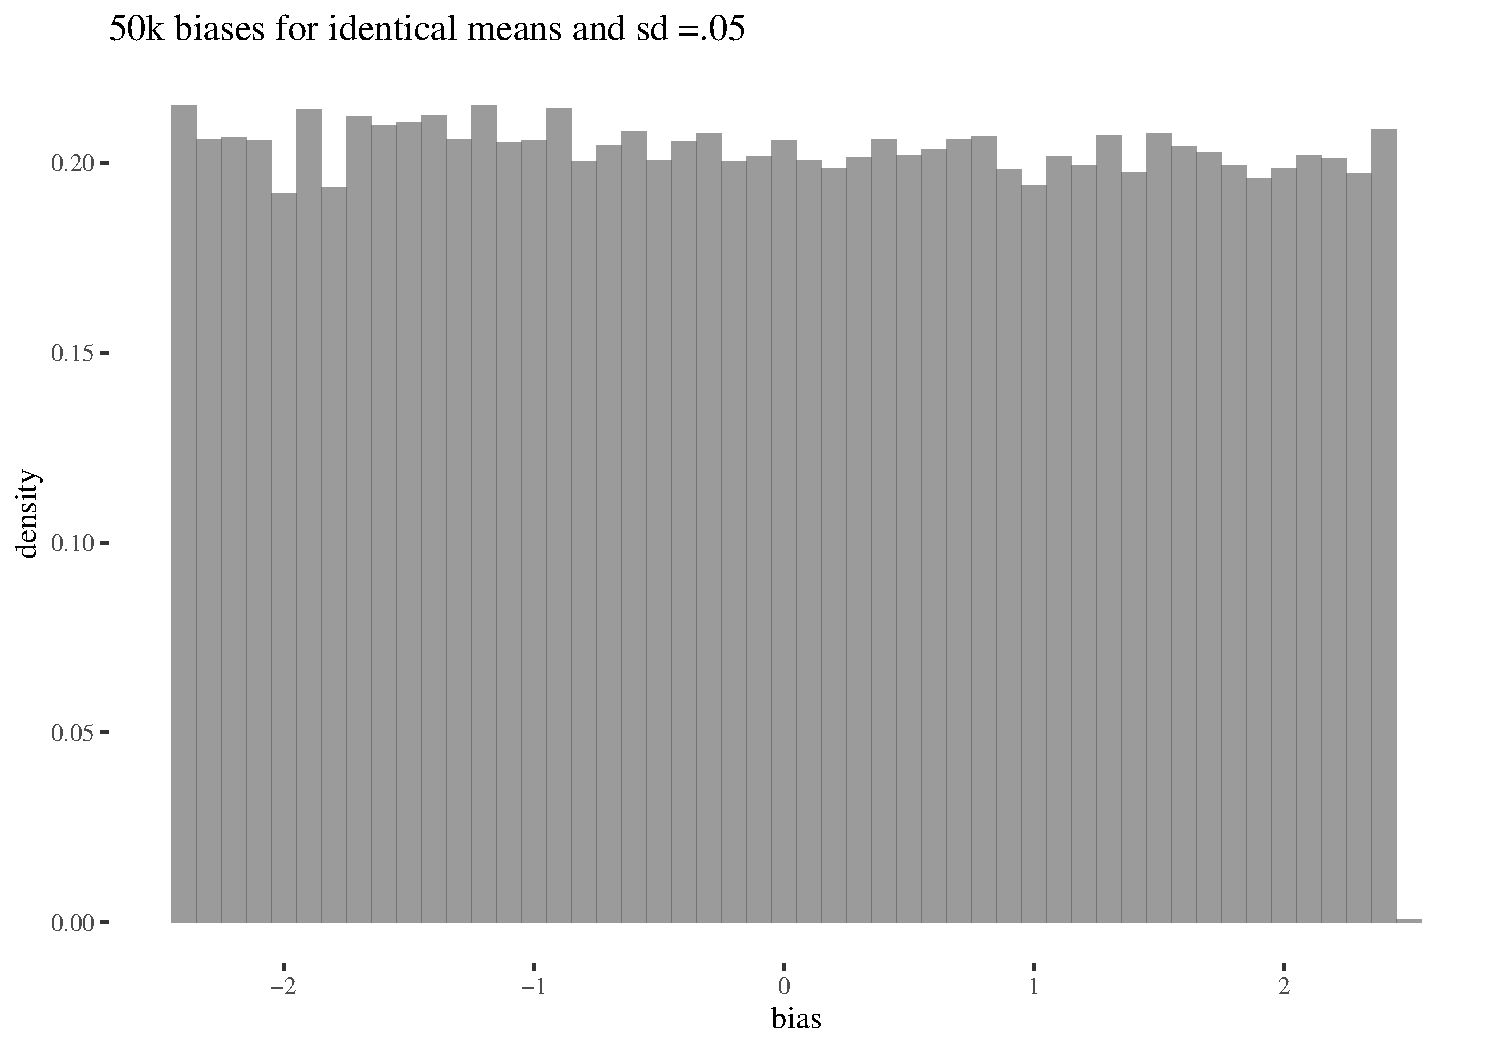
\includegraphics[width=0.8\linewidth]{presentationESSLLI_files/figure-beamer/unnamed-chunk-8-1} \end{center}

\end{block}

\end{frame}

\begin{frame}{Advantages of the Bayesian way}

\begin{itemize}
\tightlist
\item
  Direct impact of sample sizes
\item
  Straightforward interpretation in terms of posterior probabilities
\item
  Freedom to choose granularity level
\item
  More honest risk assessment and decision making
\end{itemize}

\end{frame}

\begin{frame}{Bayesian model}

\begin{block}{Choosing priors}

\begin{center}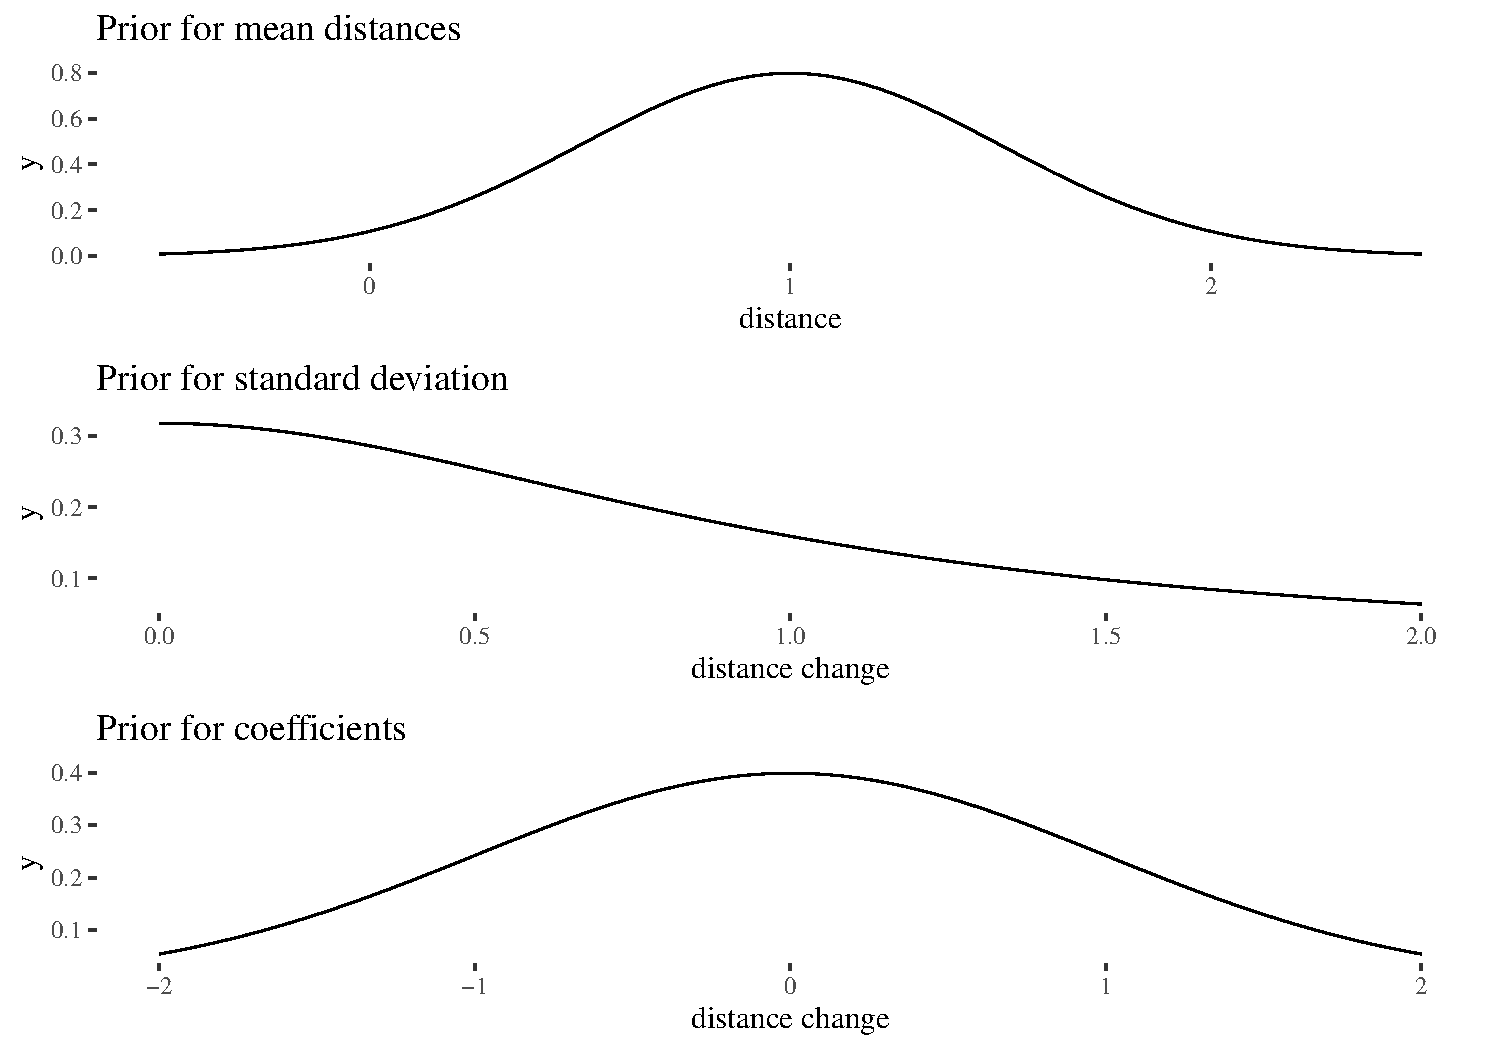
\includegraphics[width=1\linewidth]{presentationESSLLI_files/figure-beamer/priorsVis-1} \end{center}

\end{block}

\end{frame}

\begin{frame}[fragile]{Bayesian model architecture}

\vspace{1mm} \footnotesize

\begin{Shaded}
\begin{Highlighting}[]
\KeywordTok{library}\NormalTok{(rethinking)}
\KeywordTok{options}\NormalTok{(}\DataTypeTok{buildtools.check =} \ControlFlowTok{function}\NormalTok{(action) }\OtherTok{TRUE}\NormalTok{ )}
\NormalTok{religionCoefs <-}\StringTok{ }\KeywordTok{ulam}\NormalTok{(}
  \KeywordTok{alist}\NormalTok{(}
\NormalTok{    cosineDistance }\OperatorTok{~}\StringTok{ }\KeywordTok{dnorm}\NormalTok{(mu,sigma),}
\NormalTok{    mu <-}\StringTok{ }\NormalTok{m }\OperatorTok{+}\StringTok{ }\NormalTok{co[con],}
\NormalTok{    m }\OperatorTok{~}\StringTok{ }\KeywordTok{dnorm}\NormalTok{(}\DecValTok{1}\NormalTok{,.}\DecValTok{5}\NormalTok{),}
\NormalTok{    co[con] }\OperatorTok{~}\StringTok{ }\KeywordTok{dnorm}\NormalTok{(}\DecValTok{0}\NormalTok{,.}\DecValTok{5}\NormalTok{),}
\NormalTok{    sigma }\OperatorTok{~}\StringTok{ }\KeywordTok{dcauchy}\NormalTok{(}\DecValTok{0}\NormalTok{,}\DecValTok{1}\NormalTok{)}
\NormalTok{  ),}
  \DataTypeTok{data =}\NormalTok{ religion,}
  \DataTypeTok{chains=}\DecValTok{2}\NormalTok{ , }\DataTypeTok{iter=}\DecValTok{8000}\NormalTok{ , }\DataTypeTok{warmup=}\DecValTok{1000}\NormalTok{, }
  \DataTypeTok{log_lik =} \OtherTok{TRUE}
\NormalTok{)}
\end{Highlighting}
\end{Shaded}

\normalsize

\end{frame}

\begin{frame}{Dataset-level coefficients}

\begin{block}{Religion with 89\%-compatibility intervals (HPDI)}

\begin{center}
\begin{figure}[!htb]\centering
   \begin{minipage}{0.55\textwidth}
  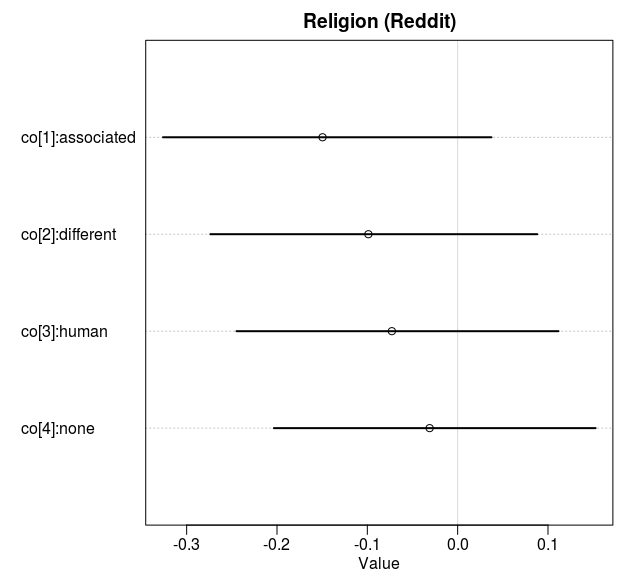
\includegraphics[width=6cm]{../images/religionCoeffs.jpeg}
   \end{minipage} \begin{minipage}{0.4\textwidth}\footnotesize
   \begin{itemize}
   \item All HPDIs overlap with 0 
   \item Differences between classes are relatively small
   \item Coefficients for Race are similar
   \end{itemize}
   \end{minipage}
  \end{figure}
  
\end{center}

\end{block}

\end{frame}

\begin{frame}{Dataset-level coefficients}

\begin{block}{Gender with 89\%-compatibility intervals (HPDI)}

\begin{center}
\begin{figure}[!htb]\centering
  \begin{minipage}{0.55\textwidth}
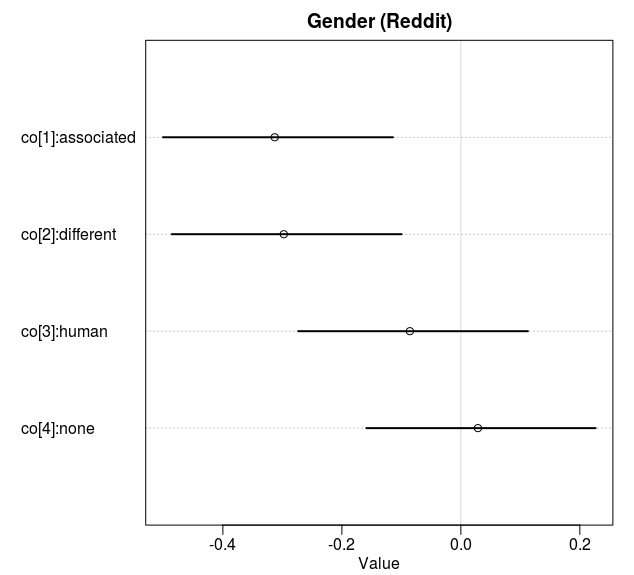
\includegraphics[width=6cm]{../images/genderCoeffs.jpeg}
\end{minipage}
\begin{minipage}{0.4\textwidth}\footnotesize
   \begin{itemize}
   \item Associated and different are away from 0
   \item But they were supposed to be opposites and are very close to each other (co-occurrence?)
   \item Differences between classes are still relatively small
   \end{itemize}
   \end{minipage}
\end{figure}


\end{center}

\end{block}

\end{frame}

\begin{frame}[fragile]{Bayesian model architecture}

\vspace{1mm} \footnotesize

\begin{Shaded}
\begin{Highlighting}[]
\KeywordTok{library}\NormalTok{(rethinking)}
\KeywordTok{options}\NormalTok{(}\DataTypeTok{buildtools.check =} \ControlFlowTok{function}\NormalTok{(action) }\OtherTok{TRUE}\NormalTok{ )}
\NormalTok{religionCoefs <-}\StringTok{ }\KeywordTok{ulam}\NormalTok{(}
  \KeywordTok{alist}\NormalTok{(}
\NormalTok{    cosineDistance }\OperatorTok{~}\StringTok{ }\KeywordTok{dnorm}\NormalTok{(mu,sigma),}
\NormalTok{    mu <-}\StringTok{ }\NormalTok{m[pw] }\OperatorTok{+}\StringTok{ }\NormalTok{co[con],}
\NormalTok{    m[pw] }\OperatorTok{~}\StringTok{ }\KeywordTok{dnorm}\NormalTok{(}\DecValTok{1}\NormalTok{,.}\DecValTok{5}\NormalTok{),}
\NormalTok{    co[con] }\OperatorTok{~}\StringTok{ }\KeywordTok{dnorm}\NormalTok{(}\DecValTok{0}\NormalTok{,.}\DecValTok{5}\NormalTok{),}
\NormalTok{    sigma }\OperatorTok{~}\StringTok{ }\KeywordTok{dcauchy}\NormalTok{(}\DecValTok{0}\NormalTok{,}\DecValTok{1}\NormalTok{)}
\NormalTok{  ),}
  \DataTypeTok{data =}\NormalTok{ religion,}
  \DataTypeTok{chains=}\DecValTok{2}\NormalTok{ , }\DataTypeTok{iter=}\DecValTok{8000}\NormalTok{ , }\DataTypeTok{warmup=}\DecValTok{1000}\NormalTok{, }
  \DataTypeTok{log_lik =} \OtherTok{TRUE}
\NormalTok{)}
\end{Highlighting}
\end{Shaded}

\normalsize

\end{frame}

\begin{frame}{Word-level coefficients}

\begin{figure}[!htb]\centering
  \begin{minipage}{0.55\textwidth}
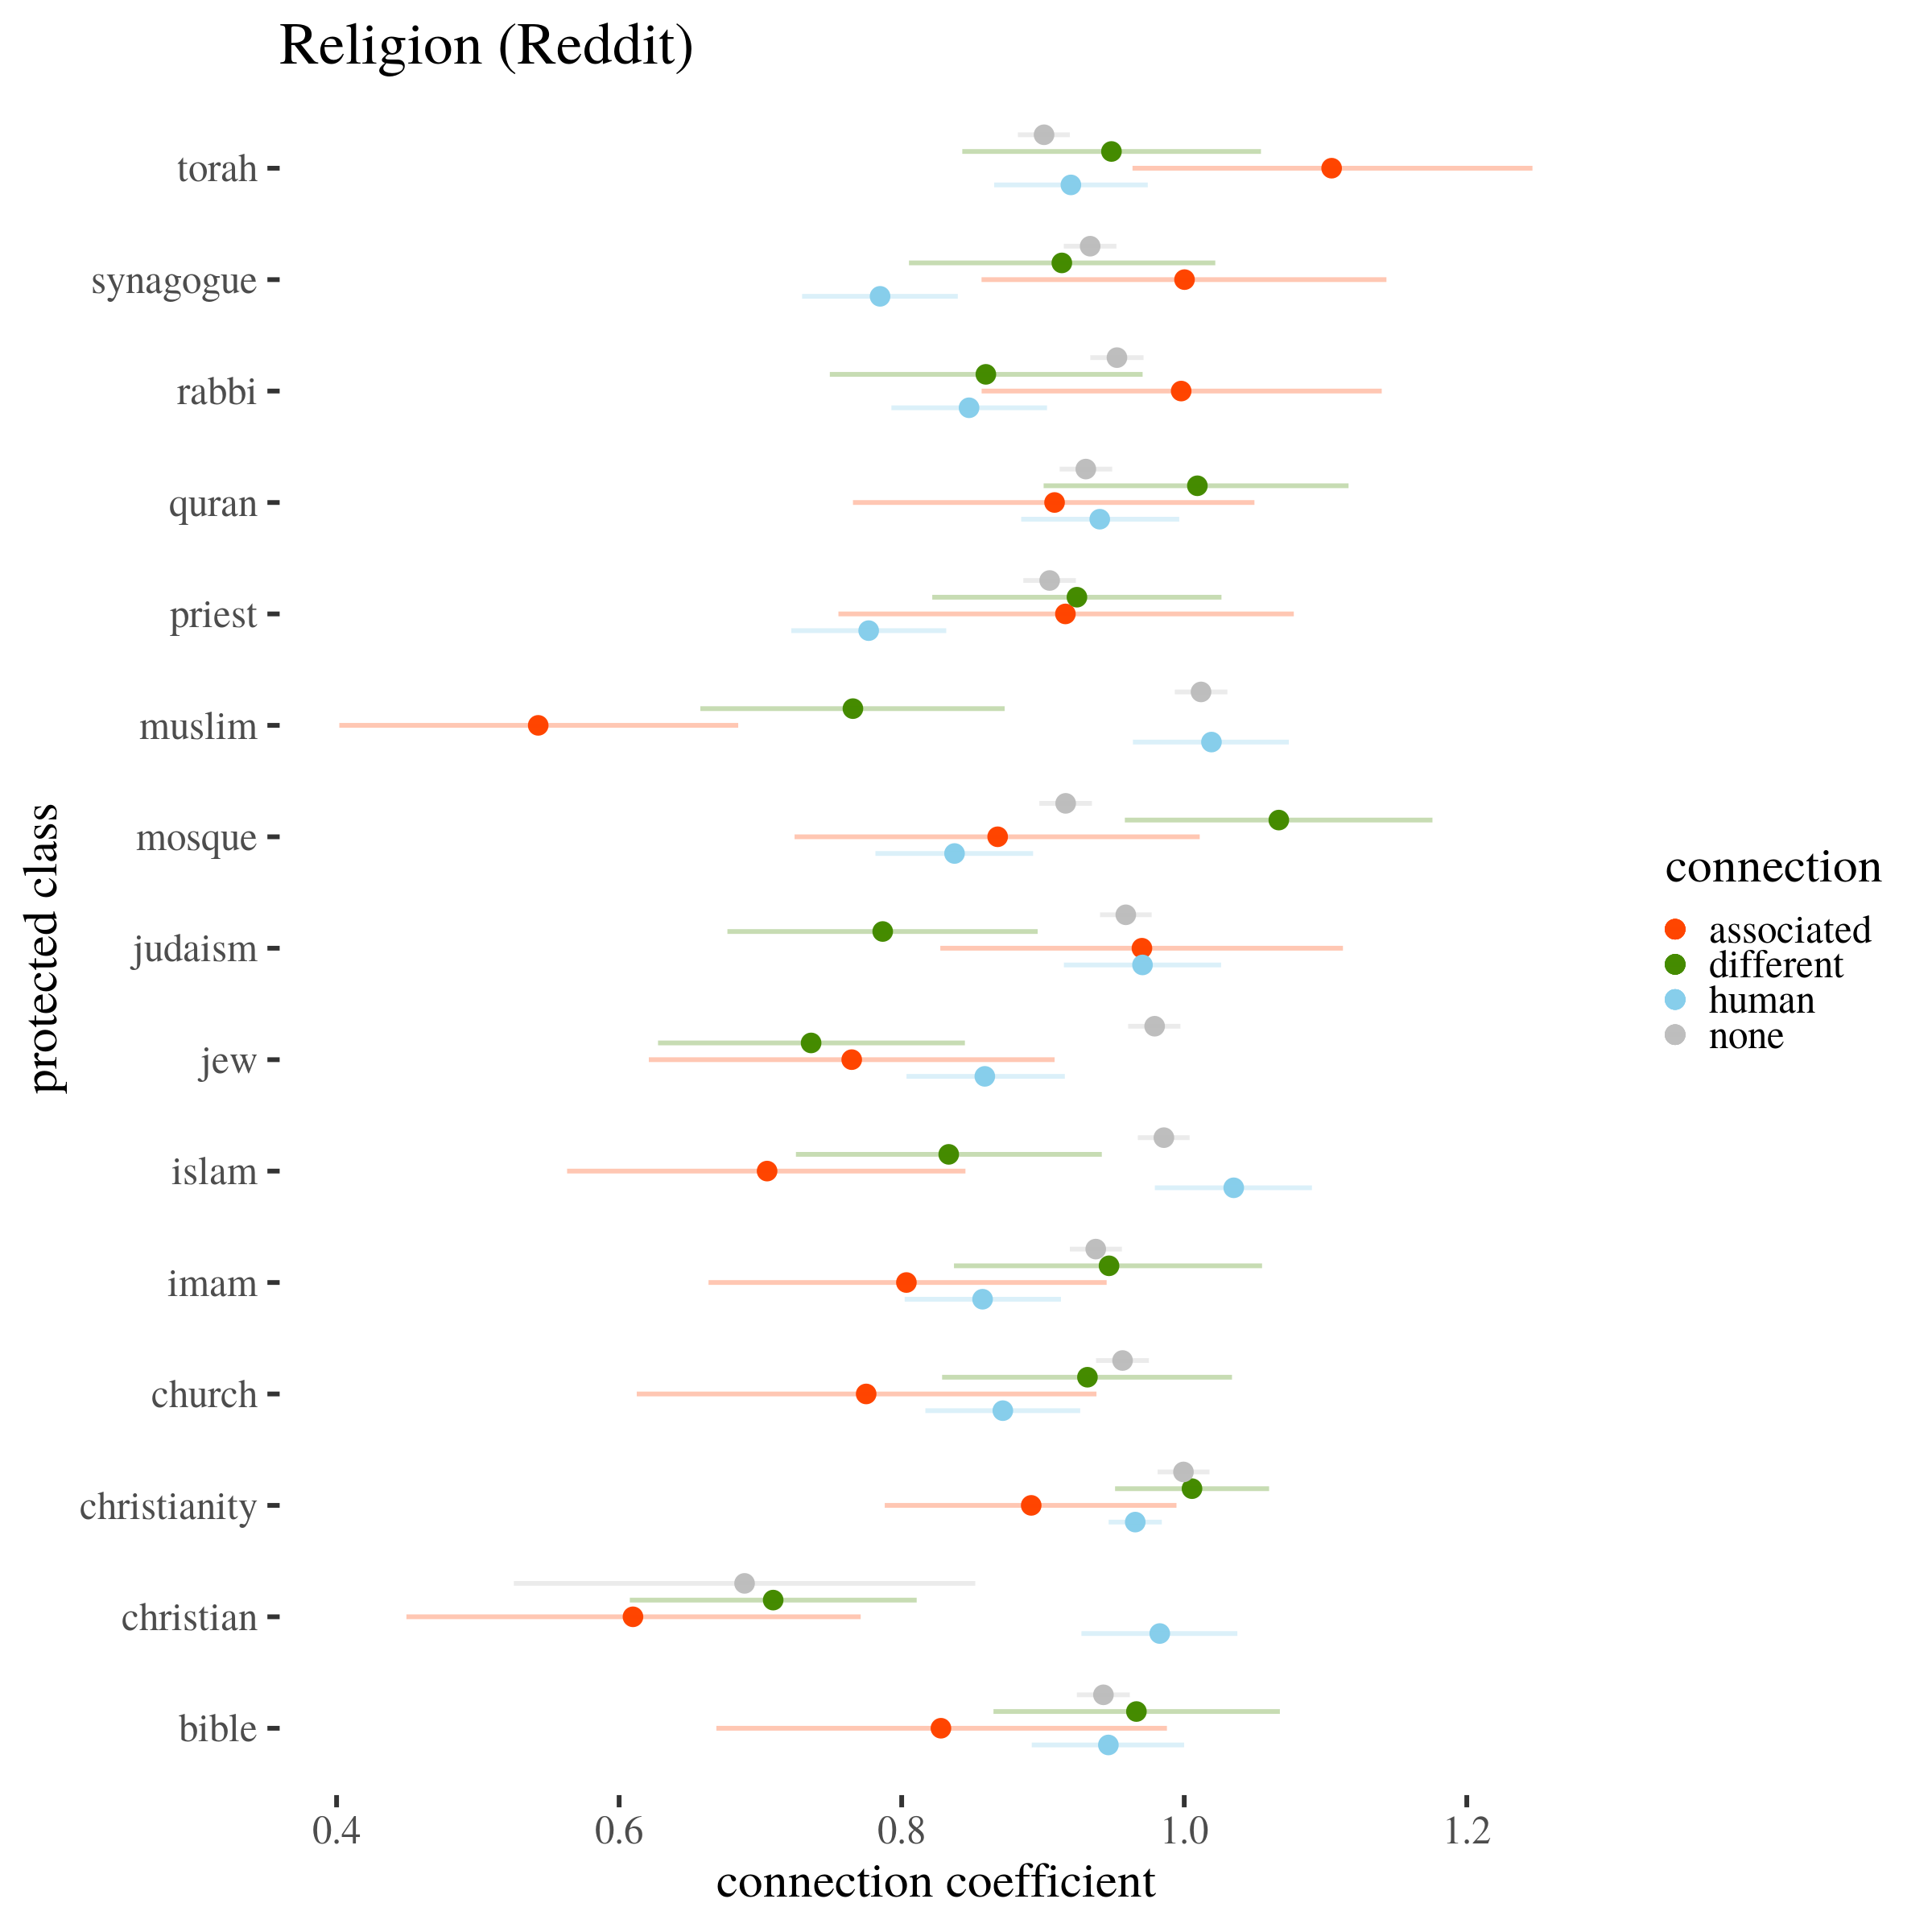
\includegraphics[width=7.5cm]{../images/visReligionReddit.png}
\end{minipage}
\begin{minipage}{0.4\textwidth}\footnotesize

\vspace{-4cm}

   \begin{itemize}
   \item Most intervals overlap with control groups
   \item Often not too much diffence between associated and different
   \end{itemize}
   \end{minipage}
\end{figure}

\end{frame}

\begin{frame}{Word-level coefficients}

\begin{figure}[!htb]\centering
  \begin{minipage}{0.55\textwidth}
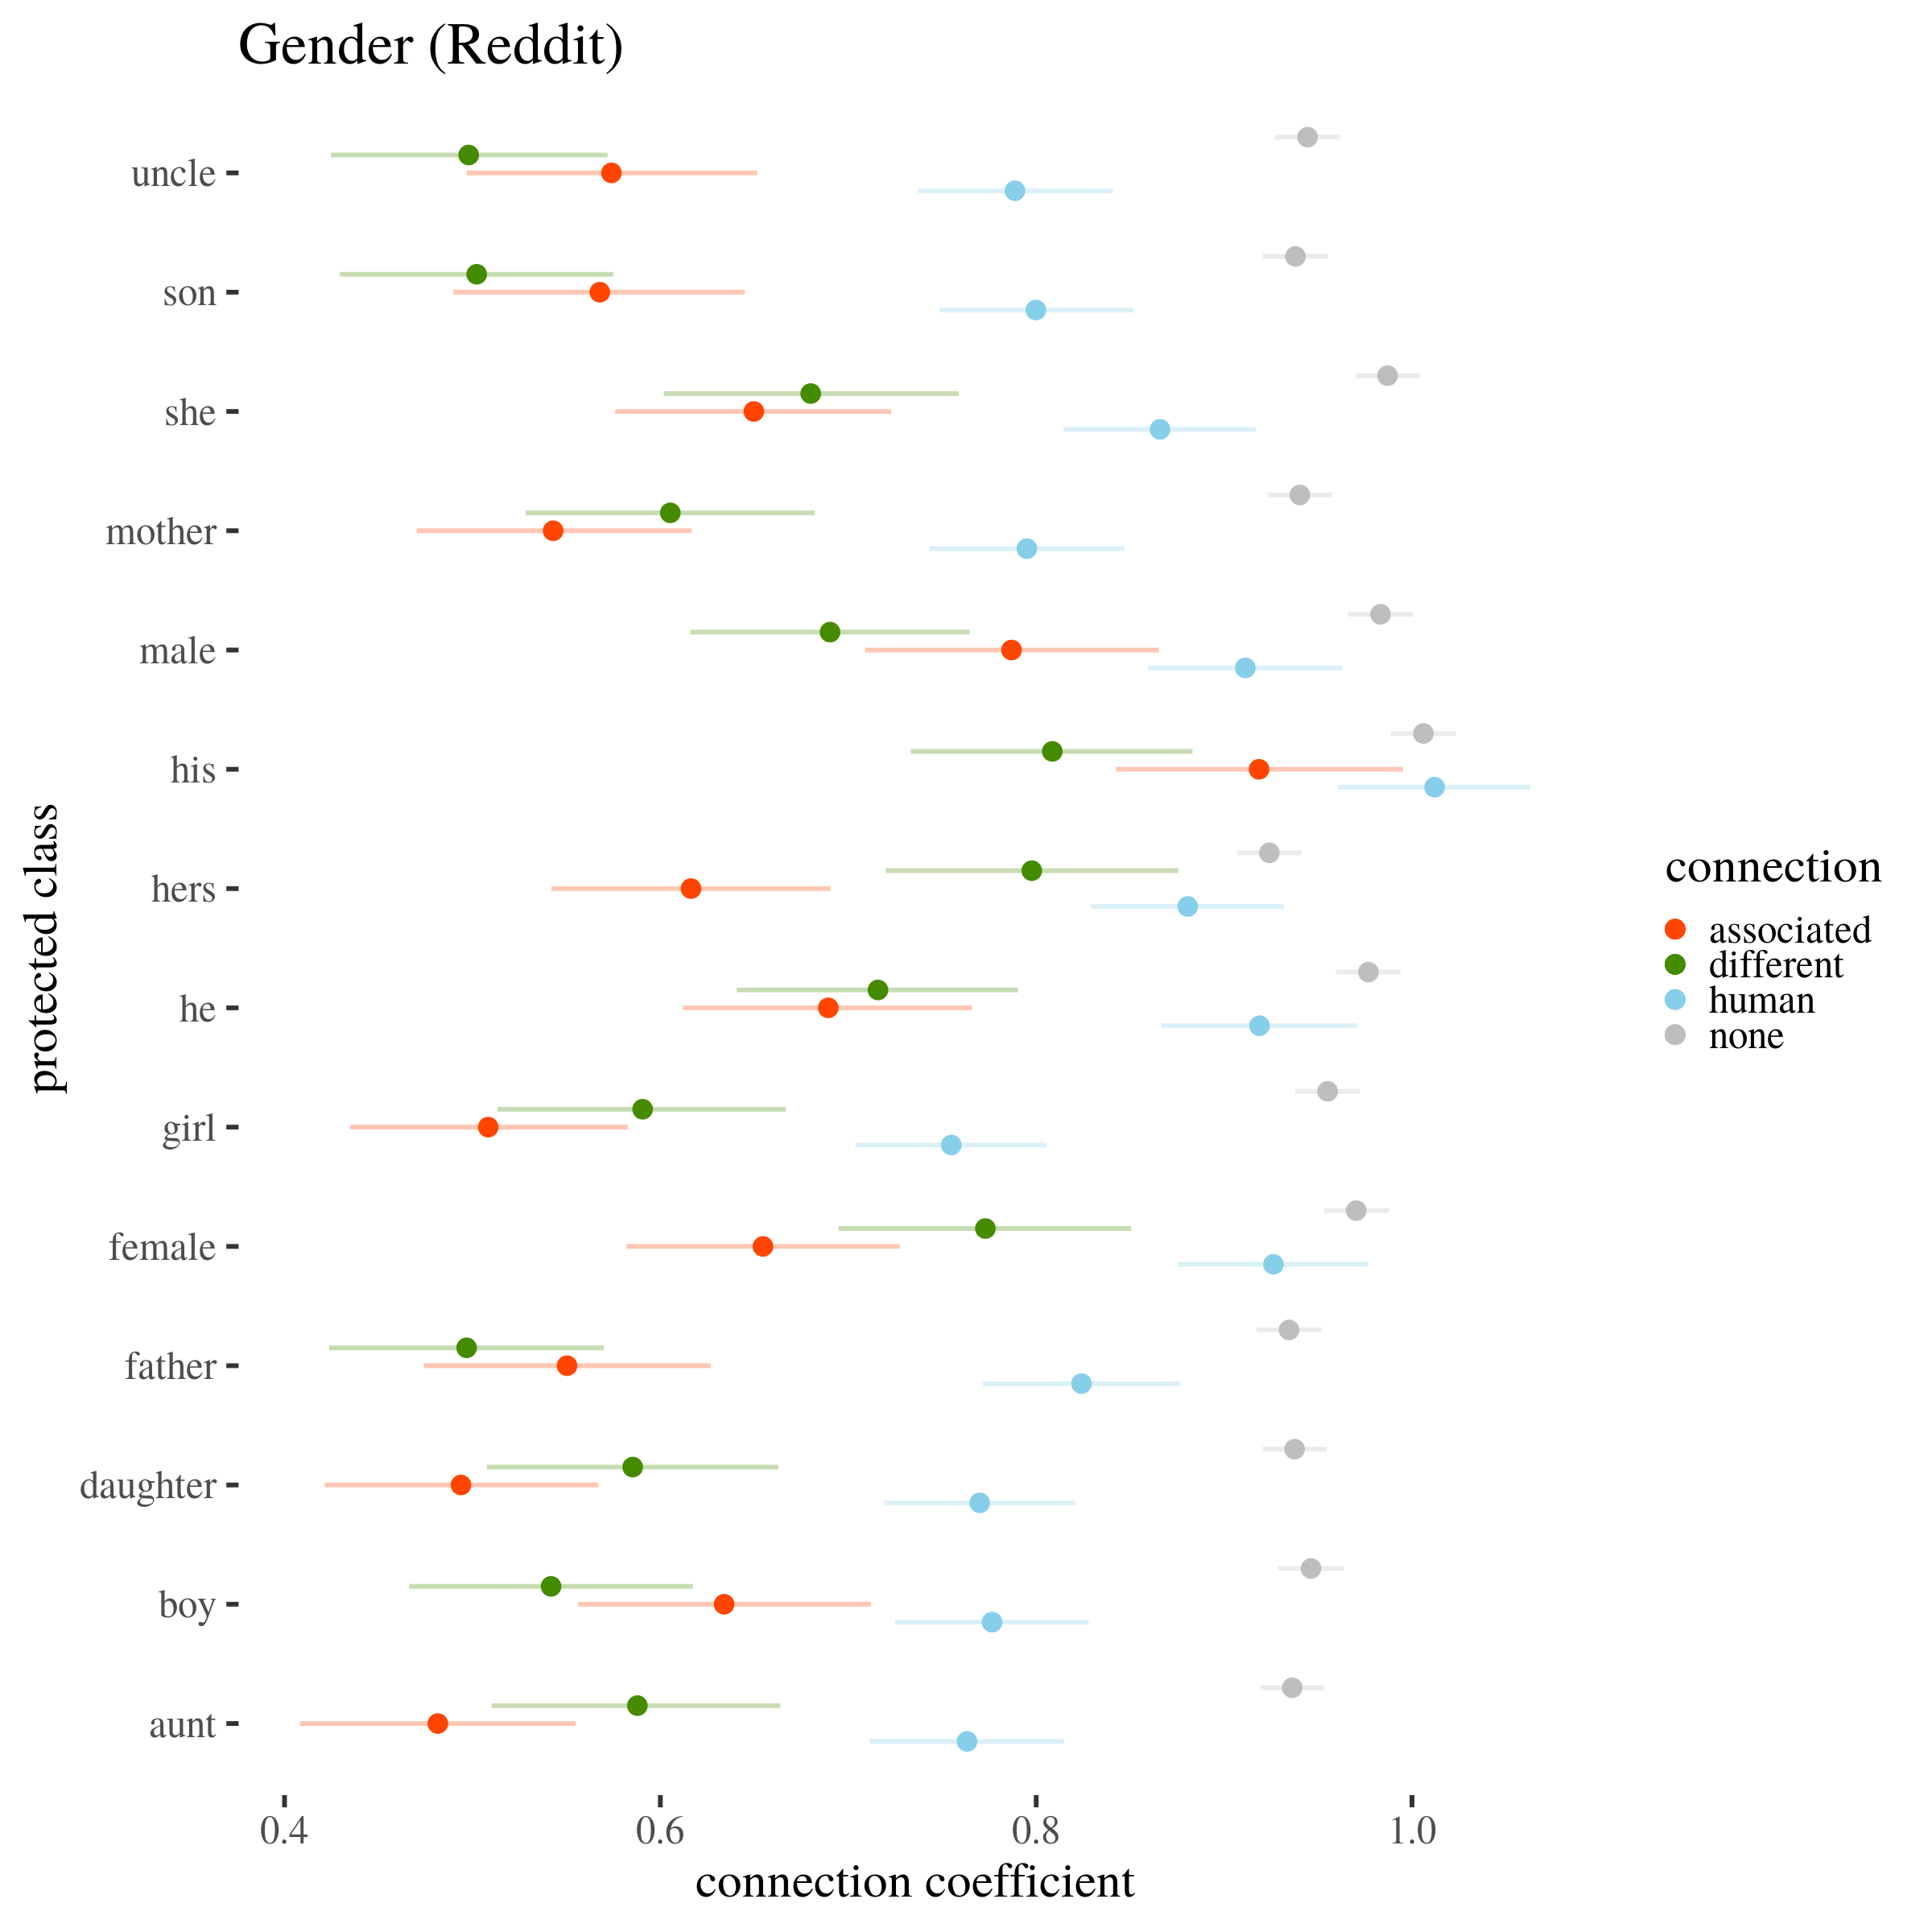
\includegraphics[width=7.5cm]{../images/visGenderReddit.png}
\end{minipage}
\begin{minipage}{0.4\textwidth}\footnotesize

\vspace{-4cm}

   \begin{itemize}
   \item Male attributes strong co-occurrence with female attributes
   \item Sometimes different is stronger than associated
   \item Almost no overlap with control groups
   \end{itemize}
   \end{minipage}
\end{figure}

\end{frame}

\begin{frame}{Word-level coefficients}

\begin{figure}[!htb]\centering
  \begin{minipage}{0.55\textwidth}
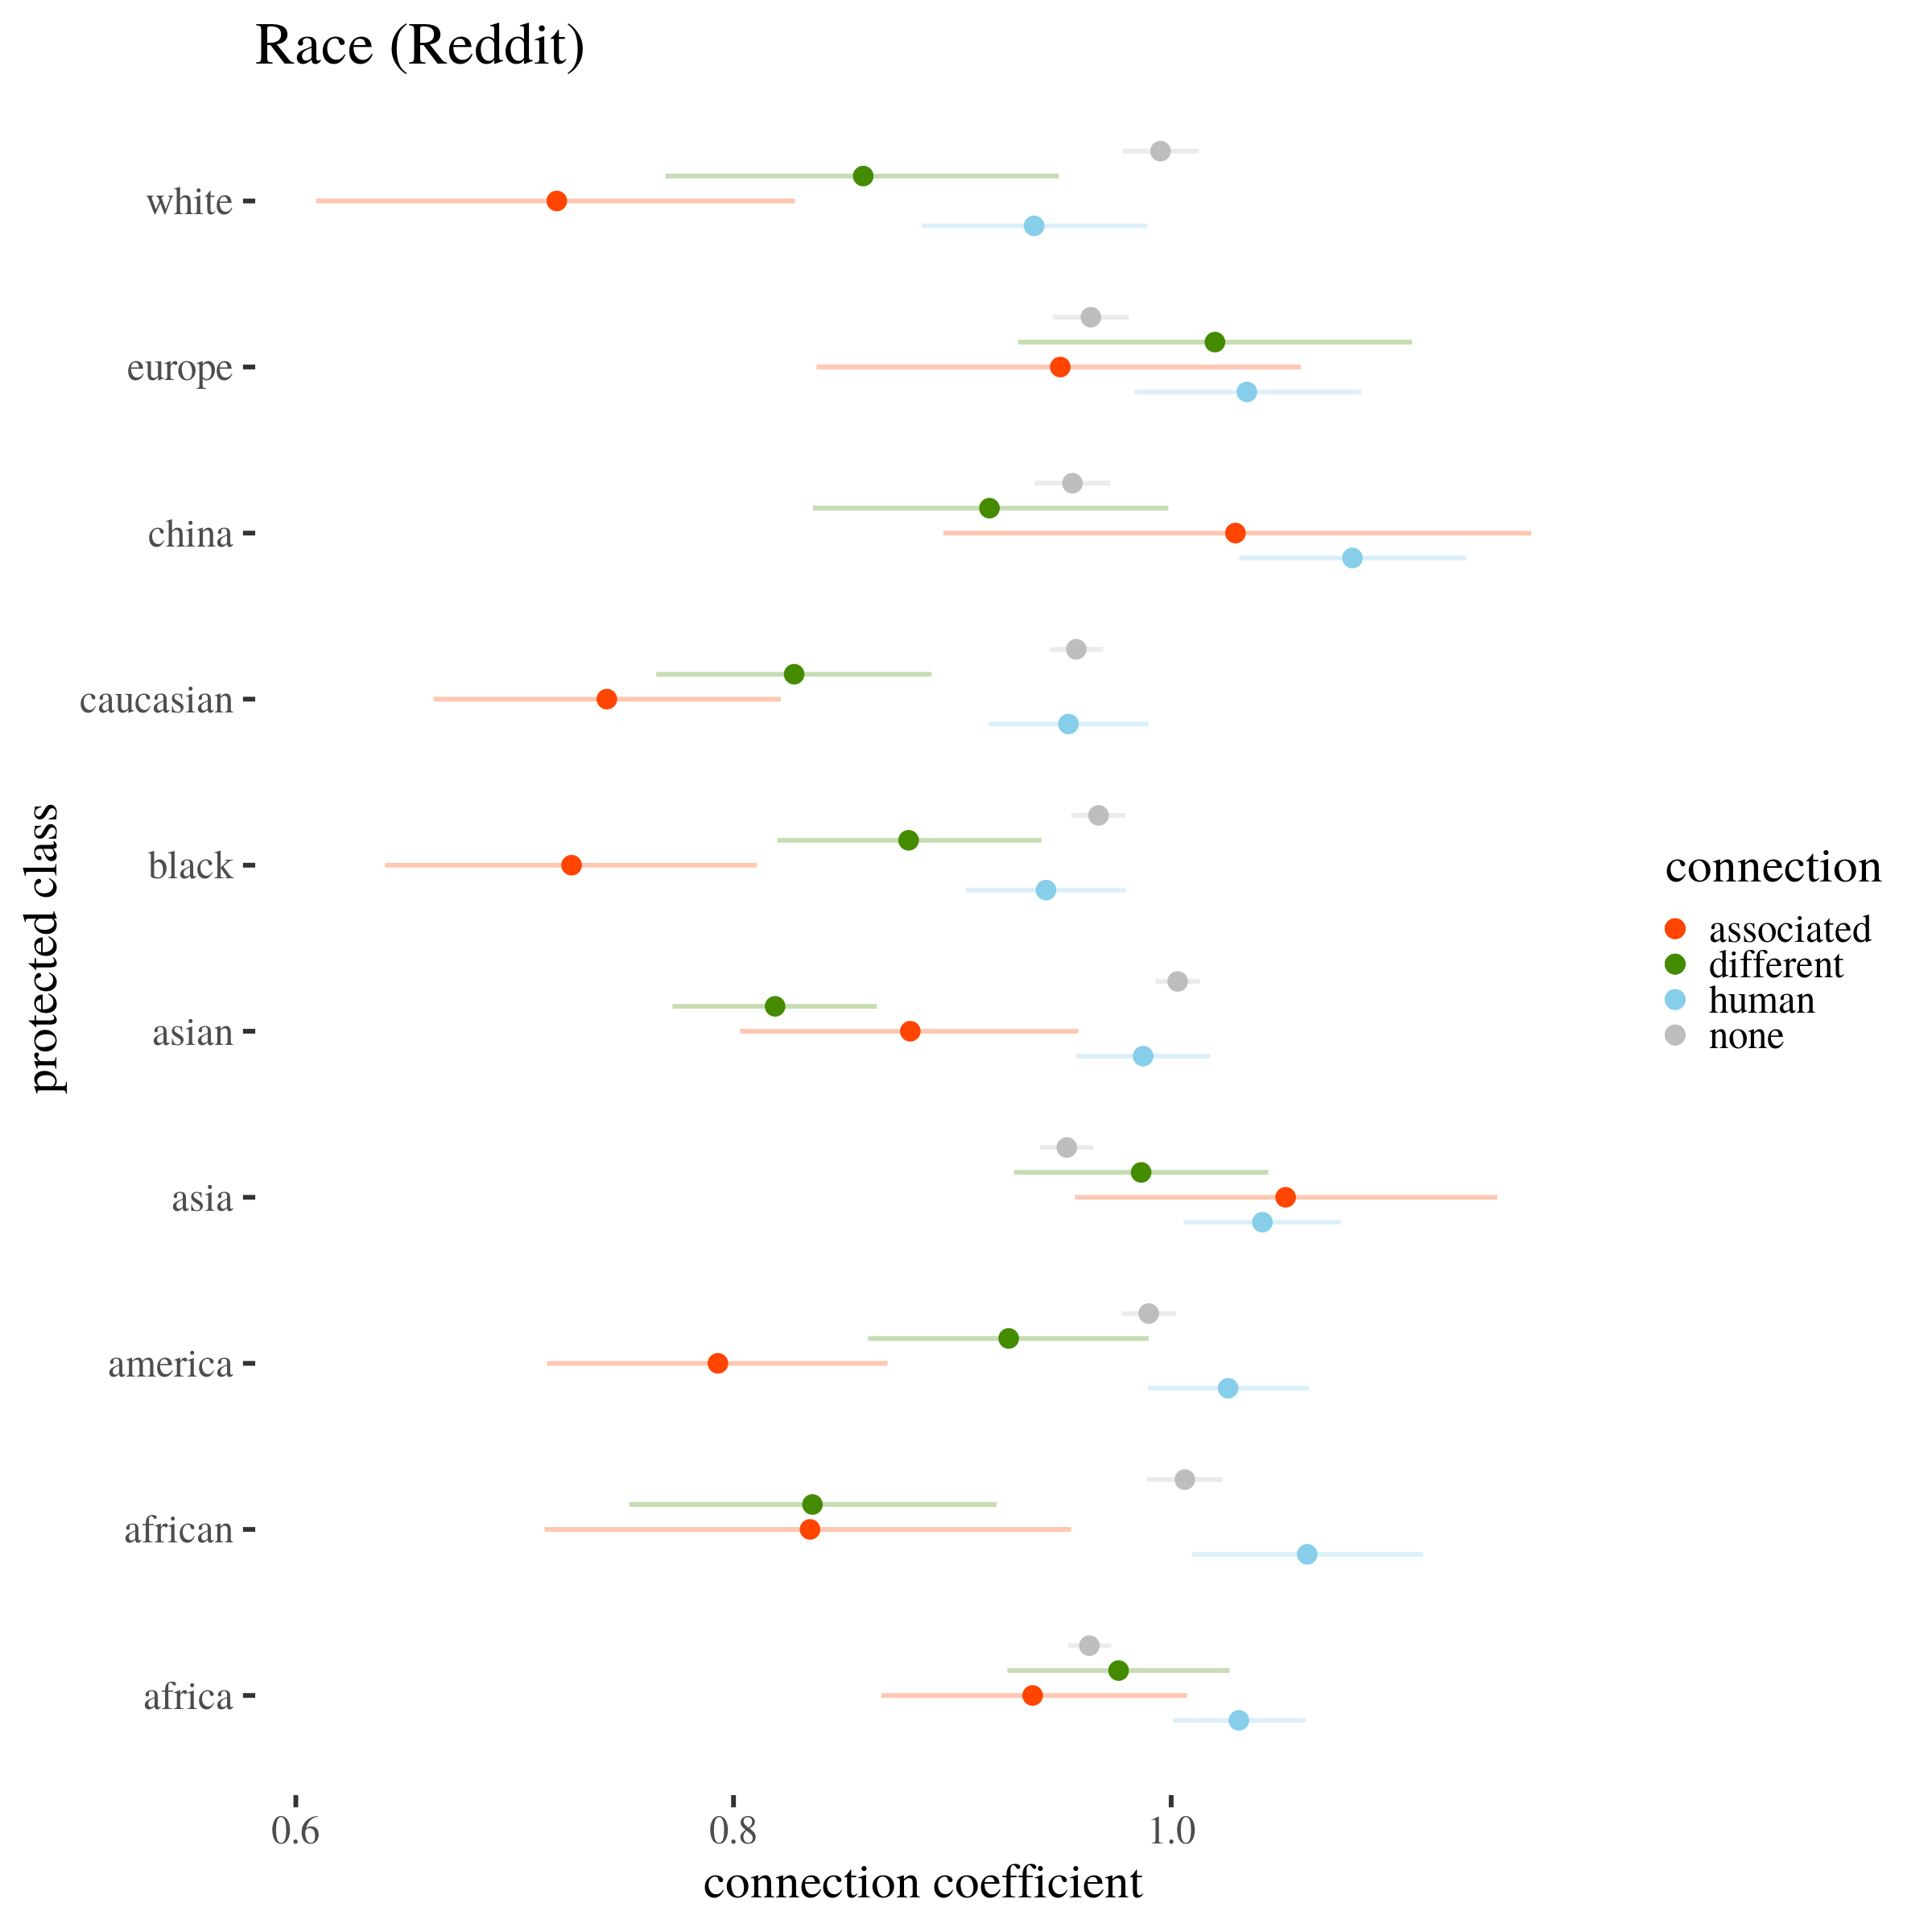
\includegraphics[width=7.5cm]{../images/visRaceReddit.png}
\end{minipage}
\begin{minipage}{0.4\textwidth}\footnotesize

\vspace{-4cm}

   \begin{itemize}
   \item A lot of variation between races
   
   \item Often not much difference between associated and different
   \end{itemize}
   \end{minipage}
\end{figure}

\end{frame}

\begin{frame}{Further work}

\begin{itemize}
\tightlist
\item
  Including contrasts in Bayesian calculation
\item
  Performance cross-validation in comparison to other methods (regular
  linear regression, KNN, \dots?)
\item
  Downstream tasks and connection with intrinsic evaluation
\item
  Testing data from the original Implicit Association Test (IAT)
\item
  Applying uncertainty to WEAT and better word lists
\item
  Looking at other similarity measures
\end{itemize}

\end{frame}

\begin{frame}{References}

\tiny

\hypertarget{refs}{}
\hypertarget{ref-Caliskan2017semanticsBiases}{}
Caliskan, A., Bryson, J. J., \& Narayanan, A. (2017). Semantics derived
automatically from language corpora contain human-like biases.
\emph{Science}, \emph{356}(6334), 183--186.
\url{https://doi.org/10.1126/science.aal4230}

\hypertarget{ref-Garg2018years}{}
Garg, N., Schiebinger, L., Jurafsky, D., \& Zou, J. (2018). Word
embeddings quantify 100 years of gender and ethnic stereotypes.
\emph{Proceedings of the National Academy of Sciences}, \emph{115}(16),
E3635--E3644. \url{https://doi.org/10.1073/pnas.1720347115}

\hypertarget{ref-Gonen2019lipstick}{}
Gonen, H., \& Goldberg, Y. (2019). Lipstick on a pig: Debiasing methods
cover up systematic gender biases in word embeddings but do not remove
them. \emph{Proceedings of the 2019 Conference of the North American
Chapter of the Association for Computational Linguistics: Human Language
Technologies, Volume 1 (Long and Short Papers)}, 609--614. Minneapolis,
Minnesota: Association for Computational Linguistics.
\url{https://doi.org/10.18653/v1/N19-1061}

\hypertarget{ref-Lauscher2019multidimensional}{}
Lauscher, A., \& Glavas, G. (2019). Are we consistently biased?
Multidimensional analysis of biases in distributional word vectors.
\emph{CoRR}, \emph{abs/1904.11783}. Retrieved from
\url{http://arxiv.org/abs/1904.11783}

\hypertarget{ref-Manzini2019blackToCriminal}{}
Manzini, T., Lim, Y. C., Tsvetkov, Y., \& Black, A. W. (2019).
\emph{Black is to criminal as caucasian is to police: Detecting and
removing multiclass bias in word embeddings}.

\hypertarget{ref-Nissim2020fair}{}
Nissim, M., Noord, R. van, \& Goot, R. van der. (2020). Fair is better
than sensational: Man is to doctor as woman is to doctor.
\emph{Computational Linguistics}, \emph{46}(2), 487--497.
\url{https://doi.org/10.1162/coli_a_00379}

\hypertarget{ref-zhang2020robustness}{}
Zhang, H., Sneyd, A., \& Stevenson, M. (2020). \emph{Robustness and
reliability of gender bias assessment in word embeddings: The role of
base pairs}.

\end{frame}

\end{document}
